\chapter{动植物选择}
\label{chp:plant:begin}

\section{主要作物的选择}
由于在火星表面的尘土里含有大量的硫酸盐和氯化物盐,这是液态水曾经存在的证据,但同时也意味着加水后土壤会呈现较强的酸性。总的来说土豆喜欢偏弱酸性的土壤,因此还算是一种不错的火星作物的候选者。但如果pH值低于4.8,土豆就不能正常生长了。

种植土豆,从芽开始算起15天成苗、用20天长匍匐茎、用30天成块,基本两个多月就能收。而且它也容易种容易收,只要切成块,埋到土里就能长。唯一的要求是每个切块上必须要有芽眼。

植物发生不可逆的永久萎蔫时的土壤含水率。这个值因土壤类型不同而有很大差异,比如说砂土是1.8--4.2\%,粘土是17.4--24\%。土壤里的水含量比这些值低,植物就会干死。

根据每立方米土壤需要40升水灌溉。这40升水指的是“土壤有效水分”,必须浇在含水量高于萎蔫系数的土里才能被植物利用。对于原本不含液态水的火星土,每立方米40升水也就是大约1.4\%的含水量,哪怕是砂质土最低的萎蔫系数也比这个值高。更何况火星土很大一部分是硅酸盐黏土,最终可能需要加水到土壤的15\%--20\%。即使种植土豆来供给能量也并不是一个简单的工作。

同时要让土豆长好,光有粪便里的细菌还不够。在地球上,植物根际土壤里的微生物构成了一个小小的生态系统,植物依赖这些细菌吸收养分,甚至还能利用它们传递信息。土豆对微生物的依赖倒不像兰花什么的那样极端,但缺了终归不行。

火星土含有千分之几的高氯酸盐,而火星的液态水也的确是塞满了这些东西的强力卤水。所幸,这些盐类是溶于水的,必须先用水把土漂洗一遍,反正水是可以循环的。

还有需要考虑土壤的厚度。标准的土豆种植,至少要深翻20厘米,最好30厘米,这样才能给土豆留足空间长不了多久土豆们就要纷纷“出土”了。出土倒是不会变成土豆地雷,但就会接受光照,开始积累龙葵素。

土豆有个休眠期,不是埋进去就能发芽。靠谱的办法是用赤霉素来刺激土豆,可以在5天之内发芽。但如果指望自然发芽,那一般条件都得25天——一下子凭空加了一个月的周期。所以要计算好土豆收获周期和工作人员的能量需求也是一个十分严密,不能出错的环节。

\section{其他作物的选择}
\paragraph{番茄}

我们栽培的番茄有两类:无限型番茄和矮株番茄。
番茄颜色鲜艳,富含维生素和矿物质元素,番茄红素具有独特的抗氧化能力,营养价值颇高。
番茄可生食、可入菜,酸甜可口,能给予乘员心理慰藉。
我们的栽培方法采用的是水培法,辅以人工基质固定根系。先将番茄种子发苗,再将发育好的幼苗定植到栽培槽内,接下来便是定期循环处理营养液并补加养分和水。番茄便参与到了整个生命保障系统的循环运行中。

\paragraph{油莎豆}

又名油莎草、虎坚果、油渣子、糖根果、地下板栗或地下核桃等,原产于非洲及地中海沿岸国家,属禾本科一年生植物。随着人们对油莎豆的深入研究,其又被誉为优质、高产、综合利用价值很高的油、粮多用新型作物,并被列为BLSS主要粮食作物的候选者之一,在主要作物职能是为乘员提供植物油。
下面分析选择油莎豆作为油料作物的原因。

首先,油莎豆相较于其他油料作物更易栽培,对环境条件要求不苛刻。我国南北各地的沙滩、丘陵、林间等均可种植,且抗旱抗涝、易种易管,可以单种也可以与其他作物套种。其播种、管理、收获、贮藏与花生相似,喜光、好气、耐旱、抗盐碱,同时对光周期、温湿度等环境条件的要求不严格,年均气温在20\si{\degreeCelsius}以上即可。整个生长周期为130天左右,病虫害很少,是目前油料作物中产量最高的作物。

其次,油莎豆营养价值高。油莎豆含油率高达38.7\%,油质优于花生油和芝麻油,味道醇香,颜色透明,久放不变质,对降低血脂、防治心血管和肌体代谢疾病等,具有独特功效,除此之外,油莎豆还具有较高的可溶性糖(含量见\cref{fig:tigernut-nutri}),因此油莎豆生食或熟食时味道香甜,目前已有油莎豆加工而成的糕点、糖果、咖啡等。具体分析其营养成分,发现油莎豆糖分主要有蔗糖、葡萄糖、果糖、棉子糖。其功效成分主要是脂溶性的功效成分,其中VE含量为0.15\%,甾醇含量为0.53\%,说明油莎豆油脂中营养成分较高。分析油莎豆的脂肪酸组成(\cref{fig:tigernut-nutri}),油酸含量最高,出油率一般为35\%,其次是棕榈酸和亚油酸,其含量均在20\%以上,说明油莎豆油脂是不干性油,具有很好的抗氧化性,其抗氧化性高于大豆油、菜籽油、花生油等。

由此可见,油莎豆高产,有助于提高BLSS系统内植物栽培系统的空间生产效率;易于栽培和管理,有助于减少乘员对植物栽培系统的维护工作量;油脂含量高、营养价值高且含糖量高,在满足乘员对植物油所需的同时,有助于改善乘员的饮食结构和风味,进一步有助于乘员的身体健康。因此,选择油莎豆作为BLSS的主要油料作物是一种必然了。

当然,油莎豆还有一些缺点。它是采摘地下核状根茎果,果实表面有须状细根且凹凸褶皱,果皮坚硬,这些均增加了油莎豆的食用加工难度。为了便于清洗,减少清洗过程的耗水量,系统内采用水培的方式种植油莎豆。采摘后的油莎豆,可榨油,亦可干燥后食用。

\begin{figure}[H]
  \centering
  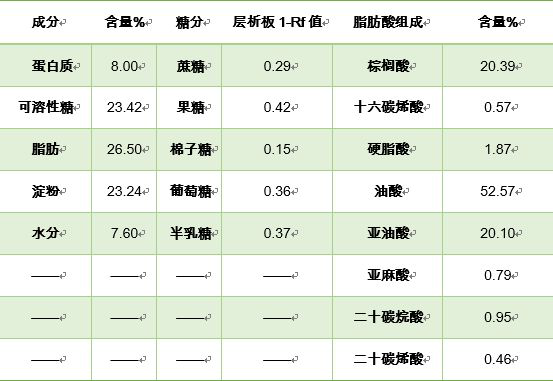
\includegraphics[width=0.8\textwidth]{figure/tigernut-nutrition.png}
  \caption{油莎豆营养成分}
  \label{fig:tigernut-nutri}
\end{figure}

\section{动物的选择}
\label{chp:plant:end}
动物方面,我们选择培养和食用黄粉虫。

作用:1. 黄粉虫是一种国际上公认的安全的可食用的虫子,黄粉虫成虫含有高达60\%的蛋白质,被誉为“蛋白质饲料宝库”,还含有磷、钾、铁等常量元素和多种微量元素,所以黄粉虫可为舱内志愿者提供动物蛋白。
2. 黄粉虫可以处理系统中部分不可食生物量,例如小麦秸秆,蔬菜的老叶子等,这样就大大增加了系统的鲁棒性。
3. 黄粉虫呼吸产生的二氧化碳,还为植物光合作用提供原料。

食用方式: 1. 将黄粉虫放置于平底锅中炒至酥脆,然后与小麦一起粉碎至面粉中,发面蒸成馒头。
2. 用植物油炒熟直接食用。
